% ============================================================
\chapter{R\'eseaux \'Equivariants et Invariants}
\label{ch:equivariants}
% ============================================================

Les r\'eseaux de neurones convolutifs doivent leur succ\`es \`a une propri\'et\'e math\'ematique pr\'ecise~: l'\'equivariance par translation. Un chat reste un chat, qu'il soit \`a gauche ou \`a droite de l'image. Mais que se passe-t-il si les sym\'etries pertinentes ne sont pas des translations~? En chimie mol\'eculaire, les propri\'et\'es d'une mol\'ecule sont invariantes par rotation et translation de l'ensemble des atomes. En physique des particules, les interactions ob\'eissent \`a des sym\'etries de jauge. Taco Cohen et Max Welling, en 2016, ont ouvert la voie des \emph{r\'eseaux \'equivariants} en montrant comment construire des couches de neurones qui respectent les sym\'etries d'un groupe donn\'e. Cette approche, formalis\'ee par le cadre g\'eom\'etrique de Bronstein et al.\, unifie les CNN, les GNN et les transformeurs comme cas particuliers d'un principe unique~: la structure du r\'eseau doit refl\'eter les sym\'etries du probl\`eme.

\section{Formalisme g\'en\'eral}

\subsection{Rappel~: \'equivariance}

\begin{definition}[\'Equivariance g\'en\'erale]
Soit $G$ un groupe agissant sur les espaces $\mathcal{X}$ et $\mathcal{Y}$
via les repr\'esentations $\rho_{\mathcal{X}}$ et $\rho_{\mathcal{Y}}$.
Une fonction $f: \mathcal{X} \to \mathcal{Y}$ est \textbf{$G$-\'equivariante} si~:
\[
    f(\rho_{\mathcal{X}}(g) \cdot x) = \rho_{\mathcal{Y}}(g) \cdot f(x),
    \quad \forall g \in G,\; \forall x \in \mathcal{X}.
\]
\end{definition}

\begin{proposition}[Composition d'applications \'equivariantes]
Si $f: \mathcal{X} \to \mathcal{Y}$ et $g: \mathcal{Y} \to \mathcal{Z}$ sont
\'equivariantes, alors $g \circ f: \mathcal{X} \to \mathcal{Z}$ est \'equivariante.
Cela justifie l'empilement de couches \'equivariantes dans un r\'eseau profond.
\end{proposition}

\subsection{Construction de couches \'equivariantes}

\begin{theoreme}[Caract\'erisation des couches lin\'eaires \'equivariantes]
L'espace des applications lin\'eaires $G$-\'equivariantes $T: V \to W$ est~:
\[
    \mathrm{Hom}_G(V, W) = \{T \in \mathrm{Lin}(V, W) :
    T \rho_V(g) = \rho_W(g) T,\; \forall g \in G\}
\]
Sa dimension est donn\'ee par le produit scalaire des caract\`eres~:
$\dim \mathrm{Hom}_G(V, W) = \inner{\chi_V}{\chi_W}_G$.
\end{theoreme}

\begin{intuition}[title=\textbf{Contrainte d'\'equivariance $=$ partage de poids}]
Imposer l'\'equivariance revient \`a \textbf{contraindre la matrice de poids}
de la couche lin\'eaire. Plus le groupe de sym\'etrie est grand, plus la
contrainte est forte, et moins il y a de param\`etres libres.
\begin{center}
\begin{tabular}{lll}
\toprule
\textbf{Groupe} & \textbf{Contrainte} & \textbf{Param\`etres} \\
\midrule
Trivial $\{e\}$ & Aucune & $n^2$ \\
Translation $\Z^d$ & Toeplitz (convolution) & $k^d$ \\
Permutation $S_n$ & Doublement stochastique & $2$ \\
$\mathrm{SO}(3)$ & Clebsch--Gordan & $\sum_k n_k m_k$ \\
\bottomrule
\end{tabular}
\end{center}
\end{intuition}

\section{R\'eseaux \'equivariants par $\mathrm{SE}(3)$}

\subsection{Motivation~: physique et chimie}

De nombreux probl\`emes physiques poss\`edent une sym\'etrie $\mathrm{SE}(3)$
(rotations + translations)~:
\begin{itemize}
    \item Pr\'ediction d'\'energie mol\'eculaire.
    \item Dynamique des prot\'eines.
    \item Simulation de fluides.
\end{itemize}

\subsection{Repr\'esentations de type $\ell$}

\begin{definition}[Champs tensoriels de type $\ell$]
Un \textbf{champ tensoriel de type $\ell$} est une fonction
$f: \R^3 \to \R^{2\ell+1}$ qui se transforme selon la repr\'esentation
irr\'eductible $D^\ell$ sous rotation~:
\[
    [L_R f](\mathbf{x}) = D^\ell(R)\, f(R^{-1}\mathbf{x})
\]
\begin{itemize}
    \item $\ell = 0$~: scalaires (1D) --- \'energie, charge.
    \item $\ell = 1$~: vecteurs (3D) --- forces, vitesses.
    \item $\ell = 2$~: tenseurs d'ordre 2 sans trace (5D) --- contraintes.
\end{itemize}
\end{definition}

\subsection{Tensor Field Networks (TFN)}

\begin{definition}[TFN --- Thomas et al., 2018]
Les \textbf{Tensor Field Networks} d\'efinissent des couches \'equivariantes
par $\mathrm{SE}(3)$ en utilisant les produits tensoriels de repr\'esentations
irr\'eductibles. Pour un n\oe ud $v$ avec position $\mathbf{r}_v$~:
\[
    \mathbf{h}_v^{\ell, (\text{out})} = \sum_{\ell_1, \ell_2}
    \sum_{u \in \mathcal{N}(v)} W^{\ell_1 \ell_2 \ell}(r_{vu})\,
    \left(\mathbf{h}_u^{\ell_1} \otimes_{\text{CG}} Y^{\ell_2}(\hat{\mathbf{r}}_{vu})\right)^\ell
\]
o\`u~:
\begin{itemize}
    \item $\hat{\mathbf{r}}_{vu} = (\mathbf{r}_v - \mathbf{r}_u) / r_{vu}$ est
          la direction normalis\'ee.
    \item $Y^{\ell_2}(\hat{\mathbf{r}})$ sont les harmoniques sph\'eriques.
    \item $\otimes_{\text{CG}}$ est le produit tensoriel avec les coefficients
          de Clebsch--Gordan.
    \item $W^{\ell_1 \ell_2 \ell}(r)$ est un noyau radial (scalaire, donc invariant).
\end{itemize}
\end{definition}

\begin{theoreme}[\'Equivariance de TFN]
Les couches TFN sont \'equivariantes par $\mathrm{SE}(3)$~: pour
$R \in \mathrm{SO}(3)$ et $\mathbf{t} \in \R^3$~:
\[
    f(R\mathbf{r}_1 + \mathbf{t}, \ldots, R\mathbf{r}_n + \mathbf{t})
    = \bigoplus_\ell D^\ell(R)\, f(\mathbf{r}_1, \ldots, \mathbf{r}_n)
\]
La preuve repose sur la propri\'et\'e de transformation des harmoniques
sph\'eriques et la d\'ecomposition de Clebsch--Gordan.
\end{theoreme}

\begin{codeblock}[title=\textbf{R\'eseau \'equivariant avec e3nn}]
\begin{minted}{python}
import torch
from e3nn import o3
from e3nn.nn.models.gate_points_2101 import Network

# Configuration du reseau
model = Network(
    irreps_in="5x0e",           # 5 scalaires en entree
    irreps_hidden="32x0e + 8x1o + 4x2e",  # representations cachees
    irreps_out="1x0e",          # 1 scalaire en sortie (energie)
    irreps_node_attr="1x0e",    # attributs de noeud
    irreps_edge_attr=o3.Irreps.spherical_harmonics(lmax=2),
    layers=3,
    max_radius=5.0,
    number_of_basis=10,
    radial_layers=2,
    radial_neurons=64,
    num_neighbors=12,
    num_nodes=20,
)

# Donnees : positions 3D et attributs
positions = torch.randn(20, 3)
node_features = torch.randn(20, 5)
node_attrs = torch.ones(20, 1)

# Verification de l'equivariance
R = o3.rand_matrix()  # rotation aleatoire
out_original = model({"node_input": node_features,
                       "positions": positions,
                       "node_attrs": node_attrs})
out_rotated = model({"node_input": node_features,
                      "positions": positions @ R.T,
                      "node_attrs": node_attrs})
print(f"Invariance scalaire: "
      f"{torch.allclose(out_original, out_rotated, atol=1e-4)}")
\end{minted}
\end{codeblock}

\section{EGNN~: \'Equivariance simplifi\'ee}

\begin{definition}[EGNN --- Satorras et al., 2021]
Les \textbf{E(n) Equivariant Graph Neural Networks} (EGNN) sont une
architecture simplifi\'ee qui atteint l'\'equivariance par $\mathrm{E}(n)$
\textbf{sans} utiliser les repr\'esentations irr\'eductibles~:
\begin{align}
    \mathbf{m}_{ij} &= \phi_e(\mathbf{h}_i, \mathbf{h}_j, d_{ij}^2, a_{ij}) \\
    \mathbf{h}_i' &= \phi_h\!\left(\mathbf{h}_i, \sum_{j \neq i} \mathbf{m}_{ij}\right) \\
    \mathbf{x}_i' &= \mathbf{x}_i + \sum_{j \neq i} (\mathbf{x}_i - \mathbf{x}_j)\,
    \phi_x(\mathbf{m}_{ij})
\end{align}
o\`u $d_{ij} = \norm{\mathbf{x}_i - \mathbf{x}_j}$ et $\phi_e, \phi_h, \phi_x$
sont des MLP.
\end{definition}

\begin{proposition}[\'Equivariance de l'EGNN]
\begin{enumerate}
    \item Les \textbf{attributs scalaires} $\mathbf{h}_i$ sont
          \textbf{invariants} par $\mathrm{E}(n)$.
    \item Les \textbf{coordonn\'ees} $\mathbf{x}_i$ sont
          \textbf{\'equivariantes} par $\mathrm{E}(n)$.
    \item La preuve repose sur le fait que $d_{ij}^2$ et
          $\mathbf{x}_i - \mathbf{x}_j$ se transforment correctement.
\end{enumerate}
\end{proposition}

\begin{codeblock}[title=\textbf{Impl\'ementation EGNN}]
\begin{minted}{python}
import torch
import torch.nn as nn

class EGNNLayer(nn.Module):
    """Couche E(n) equivariante."""
    def __init__(self, node_dim, hidden_dim):
        super().__init__()
        self.phi_e = nn.Sequential(
            nn.Linear(2 * node_dim + 1, hidden_dim),
            nn.SiLU(),
            nn.Linear(hidden_dim, hidden_dim),
        )
        self.phi_h = nn.Sequential(
            nn.Linear(node_dim + hidden_dim, hidden_dim),
            nn.SiLU(),
            nn.Linear(hidden_dim, node_dim),
        )
        self.phi_x = nn.Sequential(
            nn.Linear(hidden_dim, hidden_dim),
            nn.SiLU(),
            nn.Linear(hidden_dim, 1),
        )

    def forward(self, h, x, edge_index):
        row, col = edge_index
        # Distances au carre (invariant)
        diff = x[row] - x[col]
        dist_sq = (diff ** 2).sum(dim=-1, keepdim=True)
        # Messages
        m = self.phi_e(torch.cat([h[row], h[col], dist_sq], dim=-1))
        # Aggregation pour h
        agg = torch.zeros_like(h)
        agg.index_add_(0, row, m)
        h_new = h + self.phi_h(torch.cat([h, agg], dim=-1))
        # Mise a jour des positions (equivariante)
        x_weights = self.phi_x(m)
        x_agg = torch.zeros_like(x)
        x_agg.index_add_(0, row, diff * x_weights)
        x_new = x + x_agg
        return h_new, x_new

# Test d'equivariance
layer = EGNNLayer(32, 64)
h = torch.randn(10, 32)
x = torch.randn(10, 3)
edge_index = torch.randint(0, 10, (2, 30))

h_out, x_out = layer(h, x, edge_index)

# Rotation aleatoire
R = torch.linalg.qr(torch.randn(3, 3))[0]
if R.det() < 0:
    R[:, 0] *= -1
h_rot, x_rot = layer(h, x @ R.T, edge_index)
print(f"h invariant: {torch.allclose(h_out, h_rot, atol=1e-4)}")
print(f"x equivariant: {torch.allclose(x_out @ R.T, x_rot, atol=1e-4)}")
\end{minted}
\end{codeblock}

\section{R\'eseaux invariants}

\begin{definition}[Invariants fondamentaux]
Pour construire un r\'eseau invariant par $\mathrm{E}(n)$, on peut utiliser
les \textbf{invariants fondamentaux}~:
\begin{enumerate}
    \item \textbf{Distances}~: $d_{ij} = \norm{\mathbf{x}_i - \mathbf{x}_j}$.
    \item \textbf{Angles}~: $\theta_{ijk} = \arccos\!\left(\frac{(\mathbf{x}_j - \mathbf{x}_i) \cdot
          (\mathbf{x}_k - \mathbf{x}_i)}{\norm{\mathbf{x}_j - \mathbf{x}_i}\norm{\mathbf{x}_k - \mathbf{x}_i}}\right)$.
    \item \textbf{Dihedral}~: angle entre les plans d\'efinis par $(i,j,k)$ et $(j,k,l)$.
\end{enumerate}
\end{definition}

\begin{theoreme}[Compl\'etude des invariants]
Les distances interatomiques $\{d_{ij}\}$ d\'eterminent la g\'eom\'etrie \`a
r\'eflexion pr\`es. L'ajout des angles di\`edres l\`eve l'ambigu\"it\'e de
r\'eflexion. Tout invariant de $\mathrm{SE}(3)$ peut s'exprimer comme
fonction des distances et des angles.
\end{theoreme}

\begin{definition}[SchNet --- Sch\"utt et al., 2018]
SchNet utilise les distances interatomiques comme seule information
g\'eom\'etrique~:
\[
    \mathbf{h}_i^{(\ell+1)} = \mathbf{h}_i^{(\ell)} + \sum_{j \in \mathcal{N}(i)}
    \mathbf{W}^{(\ell)} \mathbf{h}_j^{(\ell)} \odot \text{RBF}(d_{ij})
\]
o\`u $\text{RBF}(d) = [\exp(-\gamma_1(d - \mu_1)^2), \ldots, \exp(-\gamma_K(d - \mu_K)^2)]$
est une base de fonctions radiales.
\end{definition}

\section{Hi\'erarchie de mod\`eles \'equivariants}

\begin{figure}[htbp]
\centering
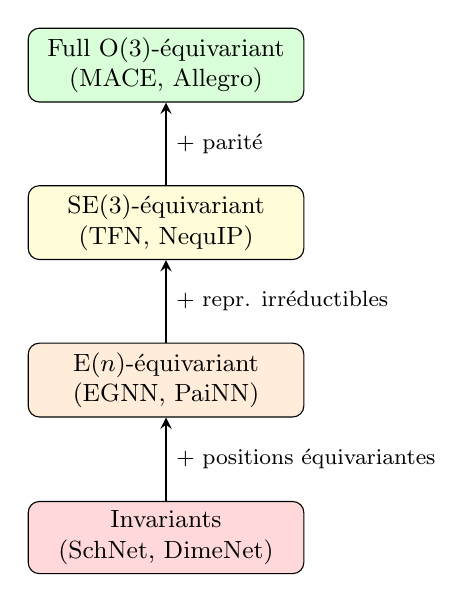
\begin{tikzpicture}[
    box/.style={rectangle, draw, rounded corners, fill=#1!15,
                minimum width=3.5cm, minimum height=0.9cm, align=center,
                font=\small},
    arr/.style={->, thick, >=stealth}
]
\node[box=red] (inv) at (0, 0) {Invariants\\(SchNet, DimeNet)};
\node[box=orange] (e3) at (0, 2) {$\mathrm{E}(n)$-\'equivariant\\(EGNN, PaiNN)};
\node[box=yellow] (se3) at (0, 4) {$\mathrm{SE}(3)$-\'equivariant\\(TFN, NequIP)};
\node[box=green] (full) at (0, 6) {Full $\mathrm{O}(3)$-\'equivariant\\(MACE, Allegro)};

\draw[arr] (inv) -- node[right, font=\footnotesize] {+ positions \'equivariantes} (e3);
\draw[arr] (e3) -- node[right, font=\footnotesize] {+ repr. irr\'eductibles} (se3);
\draw[arr] (se3) -- node[right, font=\footnotesize] {+ parit\'e} (full);
\end{tikzpicture}
\caption{Hi\'erarchie des architectures \'equivariantes.}
\end{figure}

\section*{Exercices}

\begin{exercice}[V\'erification d'\'equivariance]
Pour chacun des mod\`eles suivants, v\'erifier num\'eriquement l'\'equivariance
en appliquant des rotations, translations et r\'eflexions al\'eatoires~:
\begin{enumerate}
    \item SchNet (invariance $\mathrm{E}(3)$).
    \item EGNN (\'equivariance $\mathrm{E}(n)$).
    \item Un TFN avec sorties vectorielles (\'equivariance $\mathrm{SE}(3)$).
\end{enumerate}
\end{exercice}

\begin{exercice}[Produits tensoriels]
\begin{enumerate}
    \item Calculer le produit tensoriel $1 \otimes 1$ pour $\mathrm{SO}(3)$
          et v\'erifier la d\'ecomposition $D^1 \otimes D^1 = D^0 \oplus D^1 \oplus D^2$.
    \item Impl\'ementer avec \texttt{e3nn} et v\'erifier.
    \item Construire une couche \'equivariante qui prend deux vecteurs et produit
          un scalaire (produit scalaire), un vecteur (produit vectoriel) et un
          tenseur d'ordre 2.
\end{enumerate}
\end{exercice}

\begin{exercice}[EGNN from scratch]
Impl\'ementer un EGNN complet pour la pr\'ediction d'\'energie mol\'eculaire sur
le dataset QM9.
\begin{enumerate}
    \item Charger QM9 depuis PyTorch Geometric.
    \item Impl\'ementer 4 couches EGNN.
    \item Entra\^iner sur la propri\'et\'e $U_0$ (\'energie interne).
    \item V\'erifier l'invariance $\mathrm{E}(3)$ de la pr\'ediction.
\end{enumerate}
\end{exercice}

\begin{exercice}[Comparaison invariant vs.\ \'equivariant]
Comparer SchNet (invariant) et EGNN (\'equivariant) sur la pr\'ediction
de forces mol\'eculaires (quantit\'e vectorielle).
\begin{enumerate}
    \item Pourquoi SchNet ne peut-il pas pr\'edire directement des forces~?
    \item Comment obtient-on les forces \`a partir d'un mod\`ele d'\'energie~?
    \item L'EGNN pr\'edit-il directement des forces \'equivariantes~?
\end{enumerate}
\end{exercice}
